%%%%%%%%%%%%%%%%%%%%%%%%%%%%%%%%%%%%%%%%%%%%%%%%%%%%%%%%
% Este é um documento que servirá de modelo para
% os relatórios feitos na disciplina Laboratório de Circuitos Lógicos
% 2020-2
%%%%%%%%%%%%%%%%%%%%%%%%%%%%%%%%%%%%%%%%%%%%%%%%%%%%%%%%%

%%%%%%%%%%%%%%%%%%%%%%%%%%%%%%%%%%%%%%%%%%%%%%%%%%%%%%%%%
% Use os diferentes diretórios para colocar os relatórios de cada experimento, deste modo vc consegue manter um histórico e todo material organizado em apenas um local.
% Lembre-se de mudar o Main Document no Menu!!!

\documentclass[12pt]{article}

\usepackage{sbc-template}
\usepackage[brazil,american]{babel}
\usepackage[utf8]{inputenc}

\usepackage{graphicx}
\usepackage{url}
\usepackage{float}
\usepackage{listings}
\usepackage{color}
\usepackage{todonotes}
\usepackage{algorithmic}
\usepackage{algorithm}
\usepackage{hyperref}
\usepackage{amsmath}
\usepackage{graphicx}
\usepackage{array}
\usepackage[shortlabels]{enumitem}

\sloppy


\title{Experimento 5\\
Circuitos Combinacionais: Codificador e Decodificador}

\author{Matheus Cardoso de Souza, 202033507\\
        Ualiton Ventura da Silva, 202033580\\
        Grupo G42
}

%%%% LEMBRE-SE DE MUDAR O GRUPO NA LINHA ABAIXO!!!!! %%%%%%
\address{Dep. Ciência da Computação -- Universidade de Brasília (UnB)\\
  CIC0231 - Laboratório de Circuitos Lógicos
  \email{matheus-cardoso.mc@aluno.unb.br, 202033580@aluno.unb.br}
}

\begin{document}
\maketitle

\selectlanguage{american}
 \begin{abstract}
   TODO
 \end{abstract}

\selectlanguage{brazil}
 \begin{resumo}
   O presente relatório tem como objetivo a elaboração e análise de circuitos
   codificadores e decodificadores, sendo os codificadores compostos em sua
   entrada por 10 bits e saída de 4, já os decodificadores o inverso, ou seja, 4
   bits de entrada e 10 de saída.
 \end{resumo}


\section{Introdução}
\label{sec:Introducao}

% Escreva com suas palavras o que vai ser trabalhado no experimento. Aqui temos um exemplo de como citar a bibliografia consultada \cite{boulic:91} \cite{smith:99}.

Codificadores tem como objetivo a simplificação de um conjunto de bits dados em
uma versão simplificada sem perder a informação desejada; Por exemplo, se
tivermos uma entrada de 10 bits poderíamos produzir saídas de 4 bits, mas
observa-se que somente será possível se algumas das combinações de entrada
obtiverem a mesma saída, porque para 10 bits existem $2^{10} = 1024$ combinações
e sua saída por possuir 4 bits é capaz de produzir apenas $2^{4} = 16$ saídas.
\cite{codificadores_mandelli}

Diante desse caso existem duas possibilidades: Ou de fato as saídas possuirão
alguns resultados iguais para entradas distindas; Ou para casos como estes, em
que as entradas são diferentes mas as saídas são iguais, parte destas entradas
serão desconsideradas por serem irrevelantes para o problema (vide
\cite{codificadores_e_decodificadores} para maiores informações).

Utilizando decodificadores temos o comportamento oposto ao codificador, então
para um dado conjunto de informações simplificadas ocorrerá a decomposição em
uma maior quantidade de bits; Por exemplo, para uma entrada de 4 bits poderíamos
ter uma decomposição em 10 bits, sendo esse um comportamento desejado para a
reconstituição de uma informação simplificada em sua original.

\textbf{TODO: \emph{citar como isso pode ser útil para problemas da vida real,
    mencionar o código de gray, sua conversão de decimal para binário, mencionar
    benefícios de ter um conjunto de dados expresso de forma mais compacta (4
    bits ao invés de 10), mencionar também como codificadores e decodificadores
    podem auxiliar a conversão de dados em formato eficiente para o computador
    (binário) em dados em formato legível para o ser humano (decimal). }}

\subsection{Objetivos}
\label{sec:Objetivos}

Os textos subsequentes deste relatório tem como fim a elaboração de
codificadores e decodificadores, sendo estes codificadores compostos em sua
entradas por 10 bits e saída de 4 bits, sendo expressos no código de
\emph{Gray}. Já os decodificadores serão de maneira oposta composto por entradas
de 4 bits, no código de \emph{Gray}, e tendo por saída, dados de 10 bits; Como
resultado, por ambos circuitos possuirem lógica relacionada ocorrerá a
codificação de uma informação e atráves do decodificador ocorrerá a
reconstituição da informação.

\subsection{Materiais}
\label{sec:Materiais}
Em função da natureza do ensino a distância, os presentes experimentos não foram
realizados usando-se materiais e equipamentos físicos, mas sim emulados por meio
do \href{https://www.digitalelectronicsdeeds.com/deeds.html}{Deeds}.

A seguir estão enumerados os materiais utilizados:
\begin{itemize}
    \item Componentes de Entrada (Gerador de clock e chaves de estado)
    \item Componentes de Saída
    \item Portas Lógicas \textbf{OR}, \textbf{AND}, \textbf{NOT}
\end{itemize}

\section{Procedimentos}
\label{sec:Procedimentos}
% \setcounter{subsection}{-1}

Passaremos a apresentar os experimentos requeridos.

% 2.1
\subsection{Elaboração de Codificador}\label{sec:2.1}

Para a elaboração do circuito, deve-se analisar a seguinte tabela:
\begin{table}[H]
    \centering
    \caption{Tabela Verdade para o Decodificador}
    \begin{tabular}{|c|c|c|c|c|c|c|c|c|c||c|c|c|c|}\hline
    \multicolumn{10}{|c||}{Entradas} & \multicolumn{4}{|c|}{Saídas} \\\hline
    \textbf{$e_{0}$} & \textbf{$e_{1}$} & \textbf{$e_{2}$} & \textbf{$e_{3}$} & \textbf{$e_{4}$} & \textbf{$e_{5}$} & \textbf{$e_{6}$} & \textbf{$e_{7}$} & \textbf{$e_{8}$} & \textbf{$e_{9}$} & \textbf{A} & \textbf{B} & \textbf{C} & \textbf{D} \\\hline
    1 & 0 & 0 & 0 & 0 & 0 & 0 & 0 & 0 & 0 & 0 & 0 & 0 & 0\\\hline
    0 & 1 & 0 & 0 & 0 & 0 & 0 & 0 & 0 & 0 & 0 & 0 & 0 & 1\\\hline
    0 & 0 & 1 & 0 & 0 & 0 & 0 & 0 & 0 & 0 & 0 & 0 & 1 & 1 \\\hline
    0 & 0 & 0 & 1 & 0 & 0 & 0 & 0 & 0 & 0 & 0 & 0 & 1 & 0\\\hline
    0 & 0 & 0 & 0 & 1 & 0 & 0 & 0 & 0 & 0 & 0 & 1 & 1 & 0\\\hline
    0 & 0 & 0 & 0 & 0 & 1 & 0 & 0 & 0 & 0 & 0 & 1 & 1 & 1\\\hline
    0 & 0 & 0 & 0 & 0 & 0 & 1 & 0 & 0 & 0 & 0 & 1 & 0 & 1\\\hline
    0 & 0 & 0 & 0 & 0 & 0 & 0 & 1 & 0 & 0 & 0 & 1 & 0 & 0\\\hline
    0 & 0 & 0 & 0 & 0 & 0 & 0 & 0 & 1 & 0 & 1 & 1 & 0 & 0\\\hline
    0 & 0 & 0 & 0 & 0 & 0 & 0 & 0 & 0 & 1 & 1 & 1 & 0 & 1\\\hline
    \end{tabular}\label{tab:tabela_and}
\end{table}

Sendo que '0' é codificado como '0000000001', '1' como '0000000010', \ldots,
'9' como '1000000000'. Temos que para cada 10 bits de entrada temos que somente
1 será dado como 1, por exemplo, não temos a entrada '0000000011'.

Denotando cada um dos 10 bits como
$e_{9},e_{8},e_{7},e_{6},e_{5},e_{4},e_{3},e_{2},e_{1},e_{0}$. Assim, deve-se
analisar também que cada bit também descreve seu respectivo símbolo; Por
exemplo, $e_{8}$ descreve o símbolo '8', pois, quando $e_{8}=1$ temos que todos
os outros serão iguais a 0, portanto, estaremos descrevendo o símbolo '8'.

Para maior simplicidade podemos analisar o fato de que para a saída
\textbf{$A$}, depende de somente as entradas $e_{8}$ e $e_{9}$, como cada caso
irá ocorrer de maneira individual, \textbf{$A$} poderá ser descrito como:

\begin{equation}
F_{A}(e_{8}, e_{9}) = e_{8} + e_{9}
\end{equation}

Observação, é importante atentar-se ao fato de que em casos onde o valor
selecionado não envolve '8' ou '9', obrigatoriamente $e_{8}=0$ e $e_{9}=0$,
assim, \textbf{$A$} também será igual a 0.

Utilizando raciocínio semelhante para os demais pode ser elaborado outra das
equações booleanas, temos:

\begin{equation}
F_{A}(e_{8}, e_{9}) = e_{8} + e_{9}
\end{equation}

\begin{equation}
F_{B}(e_{4},e_{5},e_{6},e_{7},e_{8},e_{9}) = e_{4}+e_{5}+e_{6}+e_{7}+e_{8}+e_{9}
\end{equation}

\begin{equation}
F_{C}(e_{2},e_{3},e_{4},e_{5}) = e_{2}+e_{3}+e_{4}+e_{5}
\end{equation}

\begin{equation}
F_{D}(e_{1},e_{2},e_{5},e_{6},e_{9}) = e_{1}+e_{2}+e_{5}+e_{6}+e_{9}
\end{equation}

\begin{figure}[H]
    \centering
    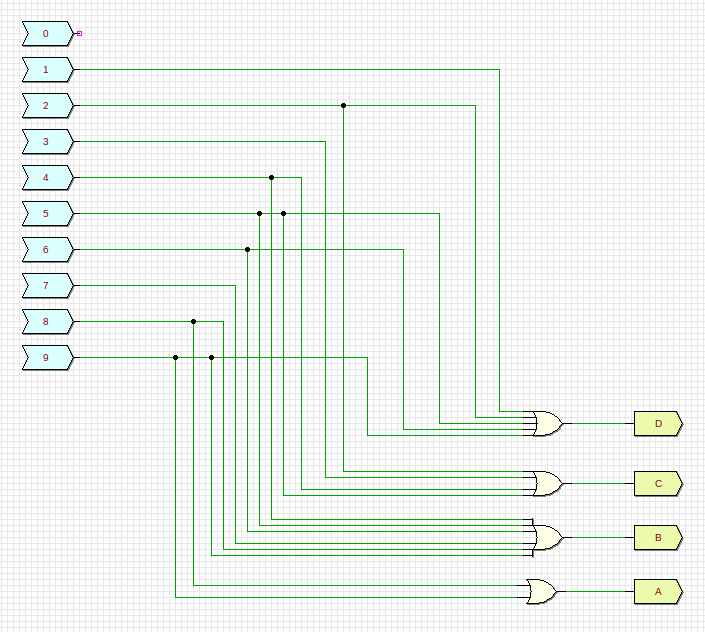
\includegraphics[width=10cm]{Exp05/2.1.png}
    \caption{Subcircuito Comparador}
    \label{fig:subComparador2.1}
\end{figure}

Importante notar que não todas as saídas são descritas, pois, possuindo 10 bits
de entrada, haverão $2^{10}$ de combinações, portanto haveriam $2^{10}$ de
saídas, contudo nos atentamos a somente algumas, todas as outras são casos não
relevantes para o problema em questão.

% 2.2
\subsection{Simulações do Codificador}\label{sec:2.2}

O diagrama esquemático será descrito por:

\begin{figure}[H]
    \centering
    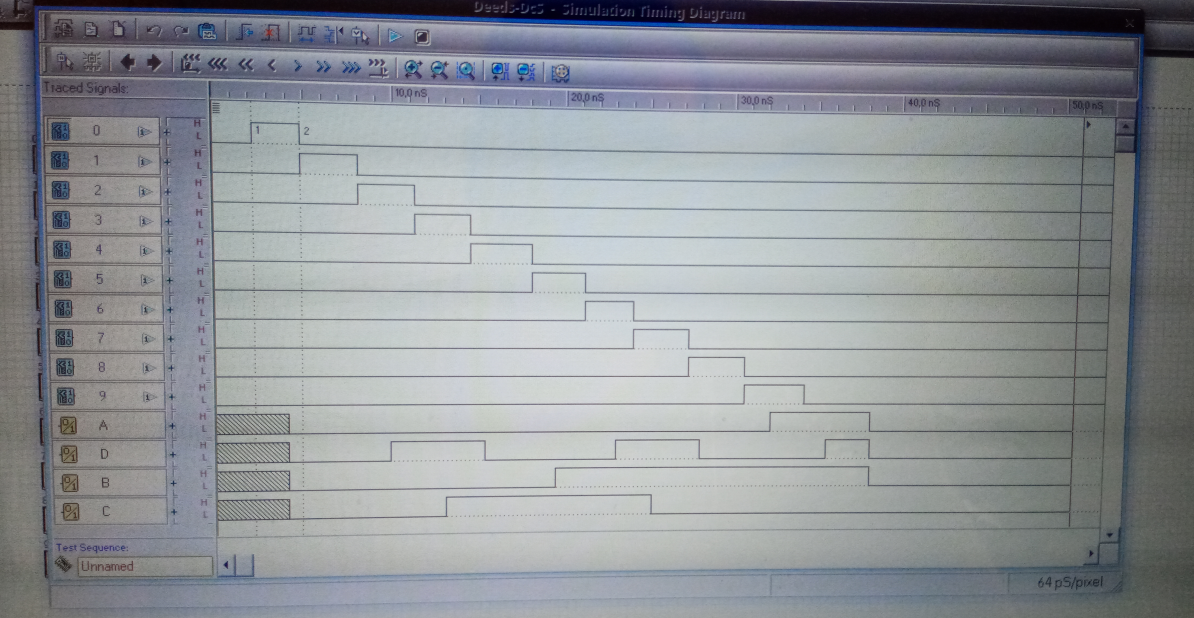
\includegraphics[width=12cm]{Exp05/2.2.png}
    \caption{TODOOOOOOOOOOOO COLOCAR CAPTION}
    \label{fig:2.2.png}
\end{figure}

Para conferir o vídeo deste experimento, acesse o seguinte link:
\href{https://youtu.be/x9ct4AeliNU}{https://youtu.be/x9ct4AeliNU}

% 2.3
\subsection{Obtendo as funções booleanas para o decodificador}\label{sec:2.3}

Nesta seção temos por objetivo obter as funções booleanas para o decodificador
de números em código de \emph{Gray} para números em decimal.




\begin{table}[H]
    \centering
    \caption{Tabela Verdade para o Decodificador}
    \begin{tabular}{|c|c|c|c||c|c|c|c|c|c|c|c|c|c|}\hline
    \multicolumn{4}{|c||}{Entradas} & \multicolumn{10}{|c|}{Saídas} \\\hline
    \textbf{A} & \textbf{B} & \textbf{C} & \textbf{D} & \textbf{$e_{0}$} & \textbf{$e_{1}$} & \textbf{$e_{2}$} & \textbf{$e_{3}$} & \textbf{$e_{4}$} & \textbf{$e_{5}$} & \textbf{$e_{6}$} & \textbf{$e_{7}$} & \textbf{$e_{8}$} & \textbf{$e_{9}$} \\\hline
    0 & 0 & 0 & 0 & 1 & 0 & 0 & 0 & 0 & 0 & 0 & 0 & 0 & 0 \\\hline
    0 & 0 & 0 & 1 & 0 & 1 & 0 & 0 & 0 & 0 & 0 & 0 & 0 & 0 \\\hline
    0 & 0 & 1 & 1 & 0 & 0 & 1 & 0 & 0 & 0 & 0 & 0 & 0 & 0 \\\hline
    0 & 0 & 1 & 0 & 0 & 0 & 0 & 1 & 0 & 0 & 0 & 0 & 0 & 0 \\\hline
    0 & 1 & 1 & 0 & 0 & 0 & 0 & 0 & 1 & 0 & 0 & 0 & 0 & 0 \\\hline
    0 & 1 & 1 & 1 & 0 & 0 & 0 & 0 & 0 & 1 & 0 & 0 & 0 & 0 \\\hline
    0 & 1 & 0 & 1 & 0 & 0 & 0 & 0 & 0 & 0 & 1 & 0 & 0 & 0 \\\hline
    0 & 1 & 0 & 0 & 0 & 0 & 0 & 0 & 0 & 0 & 0 & 1 & 0 & 0 \\\hline
    1 & 1 & 0 & 0 & 0 & 0 & 0 & 0 & 0 & 0 & 0 & 0 & 1 & 0 \\\hline
    1 & 1 & 0 & 1 & 0 & 0 & 0 & 0 & 0 & 0 & 0 & 0 & 0 & 1 \\\hline
    \end{tabular}\label{tab:tabela_and}
\end{table}

Analisando a tabela verdade, é fácil verificarmos quais devem ser as funções
booleanas de cada saída. Reproduzimos em seguida cada uma delas:

\begin{align}
e_{0} &= \overline{A} \cdot \overline{B} \cdot \overline{C} \cdot \overline{D} \\
e_{1} &= \overline{A} \cdot \overline{B} \cdot \overline{C} \cdot D \\
e_{2} &= \overline{A} \cdot \overline{B} \cdot C \cdot D \\
3 &= \overline{A} \cdot \overline{B} \cdot C \cdot \overline{D} \\
e_{4} &= \overline{A} \cdot B \cdot C \cdot \overline{D} \\
e_{5} &= \overline{A} \cdot B \cdot C \cdot D \\
e_{6} &= \overline{A} \cdot B \cdot \overline{C} \cdot D \\
e_{7} &= \overline{A} \cdot B \cdot \overline{C} \cdot \overline{D} \\
e_{8} &= A \cdot B \cdot \overline{C} \cdot \overline{D} \\
e_{9} &= A \cdot B \cdot \overline{C} \cdot D
\end{align}

TODO: terminar de escrever esse tópico

% 2.4
\subsection{Decodificador}\label{sec:2.4}

\begin{figure}[htp]
    \centering
    \includegraphics[width=12cm]{Exp05/Exp5__2_4_wave.png}
    \caption{Gráfico de Onda do \emph{Decodificador}}
    \label{fig:Exp5__2_4_wave.png}
\end{figure}

Para conferir o vídeo deste experimento, acesse o seguinte link:
\href{https://youtu.be/cj7vgZDZrKo}{https://youtu.be/cj7vgZDZrKo}

% 2.5
\subsection{Coder \& Decoder}\label{sec:2.5}

Para conferir o vídeo deste experimento, acesse o seguinte link:
\href{https://youtu.be/BpFrHE5Ggb8}{https://youtu.be/BpFrHE5Ggb8}

\section{Análise dos Resultados}
\label{sec:resultados}
TODO

\subsection{Análise em \ref{sec:2.1} e \ref{sec:2.2}}\label{sec:analise2.1}

Para o item 2.1 e 2.2 temos que de fato ocorreram os resultados esperados,
concluindo que apesar da não utilização de soma de produtos e produtos de somas
ainda assim pudemos descrever o comportamento desejado.

\subsection{Análise em 2.3}\label{sec:analise2.2}
TODO

\subsection{Análise em 2.4}\label{sec:analise2.2}
TODO

\subsection{Análise em 2.5}\label{sec:analise2.2}
TODO

\section{Conclusão}
\label{sec:Conclusao}

TODO

\nocite{*}
\bibliographystyle{sbc}
\bibliography{relatorio}  %Aqui é a definição do arquivo .bib a ser usado pelas referências


\newpage
% Colocar aqui apenas as respostas dos itens da Auto-Avaliação
\section*{Auto-Avaliação}

Respostas:

\begin{table}[H]
      \begin{tabular}{|c|c|} \hline
      \textbf{A} & \textbf{B}\\
      \hline
      1 & c \\ \hline
      2 & c \\ \hline
      3 & d \\ \hline
      4 & a \\ \hline
      5 & a \\ \hline
      6 & a \\ \hline
      7 & a \\ \hline
      \end{tabular}
\end{table}


\end{document}
